\documentclass[a4paper,uplatex,a4j,dvipdfmx]{jsarticle}
\usepackage[top=25truemm,bottom=25truemm,left=25truemm,right=25truemm]{geometry}
\usepackage[jis2004]{otf}
\usepackage[dvipdfmx]{graphicx}
\usepackage[dvipdfmx]{color}
\usepackage{longtable}
\usepackage{xcolor}

\usepackage{url}
\usepackage{makeidx}
\usepackage{pifont}
\usepackage{here}
\usepackage{multirow}
\usepackage{xparse}
\usepackage{xcolor}
\usepackage{listings}
\usepackage{plext}
\usepackage{footmisc}
\usepackage{amsmath}
\usepackage{amssymb}

\usepackage{multicol}


\usepackage[backend=biber,style=ieee]{biblatex}
\bibliography{report.bib}

% ソースコード
\lstset{
  basicstyle={\ttfamily},
  identifierstyle={\small},
  commentstyle={\smallitshape},
  keywordstyle={\small\bfseries},
  ndkeywordstyle={\small},
  stringstyle={\small\ttfamily},
  frame={tb},
  breaklines=true,
  columns=[l]{fullflexible},
  numbers=left,
  xrightmargin=0zw,
  xleftmargin=3zw,
  numberstyle={\scriptsize},
  stepnumber=1,
  numbersep=1zw,
  lineskip=-0.5ex
}

\usepackage{url}


\newcommand{\cmark}{\ding{51}}%
\newcommand{\xmark}{\ding{55}}%
\newcommand{\ctext}[1]{\hbox{\textcircled{\scriptsize{#1}}}}

\NewDocumentCommand{\codeword}{v}{%
    \texttt{\textcolor{black}{#1}}%
}

\renewcommand{\lstlistingname}{ソースコード}


\begin{document}

    \section*{概要}


    \newpage

    \begin{multicols}{2}

    \section{目的}
    私は、SNS\footnote{Social Networking Service. WEB上にて, 社会的つながりを構築し, コミュニケーションを取るプラットフォーム. 代表的なサービスに, Facebook, Twitterなどがある.}中毒者である\footnote{河井ら \cite{kawai2011sns} のSNS依存尺度に基づく.}.
    その症状として, Twitter\footnote{米Twitter社が運営する, 短文を中心としたSNSサービス. \url{https://twitter.com}}を常に見ていないと落ち着かない\footnote{順に, 離脱症状・再燃現象・葛藤(Intrapersonal conflict) \cite{griffiths2005} \label{tw}}・Twitterを開き, 閉じようと思って閉じても気づくとTwitterを開き直している・Twitterのクライアントアプリを端末から削除しても, ブラウザからアクセスしてしまう\footref{tw}・常にTweetDeckが画面に表示されており, 作業に集中できない・Twitterをなかなか辞められないことに対する罪悪感を感じているも, 結局やめることができない\footref{tw}といったものがある.
    
    また, 世の中にはSNS中毒を含むインターネット中毒と思われる人が多数存在する.
    インターネット中毒の有病率は, イタリアの0.8\%から香港の26.7\%と調査によってばらつきがある\footnote{ばらつきがある理由として, 全世界的な調査が不足していることや, ネット中毒の定義・基準, 調査の方法論が確立していないことが挙げられる\cite{IAreview}. また, インターネットの利用環境は年々変化しており, これもばらつきの一つの要因になっていると考えられる.}ものの, 世界中で一定数の人々が発症している.
    
  本課題では, 私を含む多くの人々がインターネット中毒に悩んでいる状況を踏まえ, 中毒状態から脱することをサポートするため, インターネット利用をコントロールするプロキシサーバーを開発する.



    \section{概要}
    SNS依存を断ち切るために, まずは利用時間の把握をすることが必要となる. 「数分だけ使うつもりだったのに, ついつい時間が経っていた」現象を防ぐため, まずは客観的にオンラインでの活動時間を記録することが効果的とされている\cite{internetaddiction}.
    モニタリングによって時間についての問題意識を獲得したら, 実際に利用時間を減らしていく必要がある. ここで有効な手段として, 「外的ストップテクニック」と呼ばれる, 一定時間にアラームが鳴ったらオンライン活動をストップするというものがある\cite{internetaddiction}. これにより, 少しづつ時間のコントロールを取り戻していくのである.
    そこで, WEBサービスにアクセスしてから一定時間後に通信を遮断し, また一定時間が経過したら通信を再開するHTTPプロキシを実装する.
    プログラムの名前をdetox-proxyとした.
    
    \begin{figure}[H]
      \center
      
\includegraphics[width=7cm]{img/logo.eps}
      \caption{作成したロゴ \\ スイッチの記号(JIS C 0617)をアレンジした.}
    \end{figure}

    \section{HTTP(S)プロキシの仕組み}
    
    このセクションでは, HTTP/1.1における一般的なHTTPプロキシの動作原理について, 簡単に触れておく.

    プロキシは, クライアントとサーバーの通信の間に挟まり, 通信を仲介するものとして捉えるとわかりやすい.
    
    \subsection{HTTPプロキシ}
    \label{sec:http}
    まず, OSやブラウザの設定でHTTPプロキシを有効にしておく, または環境変数\codeword{HTTP_PROXY}にプロキシサーバーのアドレスを指定しておく.
    こうすると, 自動的にアプリケーションのHTTP通信がプロキシを経由するようになる.
    \begin{figure*}[tb]
      \center
      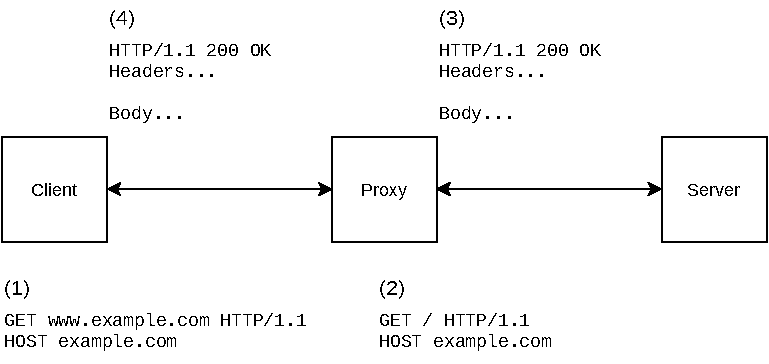
\includegraphics[width=14cm]{img/proxyhttp.pdf}
      \caption{HTTPプロキシの動作 \label{img:proxy:http}}
    \end{figure*}
    
    図\ref{img:proxy:http}に, HTTPプロキシの動作を図解した.
    まず, クライアントがプロキシに向けて, (1)のリクエストを送る.
    ここで, メソッドの隣のパスの形式は, 通常のリクエストと違い, 絶対パスとなっている. また, \codeword{HOST}ヘッダに, リクエスト先のサーバーを指定する.
    
    次に, リクエストを受け取ったプロキシは, \codeword{HOST}ヘッダに記されているアドレス宛に, (2)のリクエストを送る. ここで, 基本的にクライアントが付けたヘッダは改変せず, そのまま送信する\footnote{Forwardedヘッダ\cite{rfc:7239}など, 必要に応じてプロキシが書き換えるケースもある.}. bodyが含まれる場合は, そちらも改変せずに送信する.
    
    リクエストを受け取ったサーバーは, 通常のクライアントからのアクセスと同じように\footnote{プロキシからのアクセスなのか, 通常のクライアントからのアクセスかを見極めるのは一般的に困難である.}, (3)のレスポンスを返す. レスポンスを受け取ったプロキシは, その内容をそのままクライアントへと返す(4).
    
    このような動作で, プロキシはクライアントとサーバーとのやり取りを仲介するのである. (1)のリクエストを受け取った段階で, \codeword{HOST}ヘッダを見て通信を遮断するといったことや, (3)のレスポンスのヘッダーやボディを見て有害なものが含まれていないかチェックすると言ったことが可能となる.

    \subsection{HTTPSプロキシ}
    セクション\ref{sec:http}で紹介したHTTPプロキシの仕組みは, そのままHTTPS通信に用いることができない. なぜならHTTPS通信においては, 通信が暗号化されており, ヘッダーなどの中身をプロキシが見ることはできないからである\footnote{見たり書き換えることができてしまったら, Man-in-the-Middle攻撃になってしまう.}\footnote{なおプロキシサーバーの証明書を発行し, 通信の途中(プロキシ)で通信内容を解読し, チェックした上で再度暗号化して転送するものも存在する. 本稿では扱わない.}.
    サーバーとクライアント間のエンドツーエンド暗号化を実現しつつ, プロキシサーバーを機能させるために, HTTP/1.1では\codeword{CONNECT}メソッドが用意されている\cite{rfc:7231}.

    \begin{figure*}[tb]
      \center
      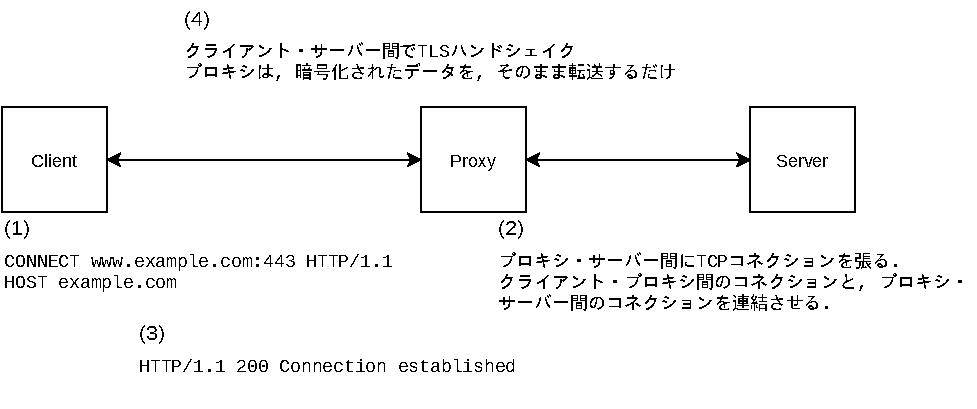
\includegraphics[width=14cm]{img/proxyhttps.pdf}
      \caption{HTTPSプロキシの動作 \label{img:proxy:https}}
    \end{figure*}
    
    図\ref{img:proxy:https}に, CONNECTメソッドを用いたプロキシの動作を示した.
    まず, クライアントはプロキシにCONNECTメソッドを使ってリクエストを送信する.
    リクエストを受け取ったプロキシは, パスに記されているサーバーのアドレス・ポートにTCPコネクションを張る. そして, これ以降クライアントから送られてきたデータは, 直接このコネクションへ流し込む. また, サーバーから送られてきたデータも, そのままクライアントとのコネクションへ流す.
    これにより, 仮想的にクライアント・サーバー間に1本のコネクションが貼られたことになる(2).
    
    その後, プロキシはクライアントへ200番台のレスポンスを返す(3).
    クライアントは, これでプロキシの先にサーバーへのコネクションが張られたとみなし, 通常のプロキシを介さないアクセスと同じ手順でTLSハンドシェイクを開始し, サーバーとセキュアな通信を行う.

    \section{仕様}
    % 全体の仕様
    
    まず, 
    
    \subsection{フロントエンド}
    
    \subsection{APIサーバー}
    
    \subsection{プロキシサーバー}
    
    

    \section{結果}

    \section{考察}
    
    まず, クライアント-プロキシ間をHTTPSで繋げるかどうかはアプリによってまちまち
    BASIC認証ができるかどうかも, アプリによってまちまち
    
    もういっそ, クライアントアプリを書こうな
    
    \section{終わりに}
    HTTPについての理解もあやふやだった自分が, 時間をかけつつも一からHTTP(S)プロキシを実装できたことに, 大変な喜びを感じている.
    ここまで紹介してきた機能の他に, クライアントとプロキシ間の接続をTLS化したり, BASIC認証を実装したりもした.
    しかし, TLSやBASIC認証については, アプリケーションによって対応がまちまち\footnote{cURL\cite{curlhttps}, Chrome\cite{chromehttps}, Firefox\cite{firefoxhttps}といったアプリケーションは対応している. その一方で, ほとんどのアプリケーションは対応の兆しを見せておらず, プロキシサーバーが407や426を返しても無反応のまま通信が途切れてしまう.}で, 安定した接続ができなかったため, コードを削除した. 本来であれば, 上記の機能を実装した上で, サービスとして公開しようと考えていたが, それが叶わず残念だった.
    今後は, TUNデバイスなどを作成してTCP・UDPのプロキシを作成することで, こうしたアプリケーションの制約を受けないようにし, サービスを実現させたい.

    \end{multicols}


  \printbibliography[title=参考文献]
\end{document}
